\hypertarget{introduction}{%
\section{Introduction}\label{introduction5}}

Epithelial structures in biology exhibit a diverse range of shapes and sizes, including curved or folded forms. Understanding these structures can be complicated, particularly in the context of developmental biology. Interestingly, the etymology of the terms "development" and "complicated" provides insight into the importance of folding and unfolding processes. "Development" comes from the Old French word "\textit{desvelopemens}," meaning "unfolding," which describes the morphogenesis of an organism. In contrast, "complicated" comes from the Latin word "\textit{com-plicare,}" meaning "folded together," which is fitting for describing the emergence of complex, folded structures in epithelial tissues.

By utilizing the MOLI tool, we can create 3D epithelial structures by inflating domes, thereby transforming a planar monolayer into a curved configuration. In this chapter, we will discuss how these structures can be made even more \textit{complicated}. %By studying the mechanics of epithelial tissue, we have discovered that the dome can be deflated into folds by rapidly depressurizing it. We will explore the process of epithelial buckling and discuss how this knowledge has enabled us to transform domes into folded structures.

\hypertarget{rapid-deflation-produces-a-buckling-instability}{%
	\section{Rapid deflation produces a buckling
		instability}\label{rapid-deflation-produces-a-buckling-instability}}


In the previous chapter, we discovered that domes subjected to constant pressure gradually inflate and eventually reach a steady state. Employing a computational framework, we interpreted that stretching induces viscoelastic stress and active tension in the tissue. To achieve a steady state, cytoskeletal remodeling dissipates viscoelastic stress, and active tension increases to counterbalance the external pressure. Consequently, the epithelial tissue exhibits the characteristics of an active viscoelastic material.

Due to this active viscoelasticity, we observed that in cyclic pressure experiments with rates faster than remodeling timescales, the tissue deflates slower than the pressure decreases. This leads to strain accumulation in subsequent cycles. Based on these findings, we wondered if starting from an inflated dome at steady state, a rapid deflation at rates faster than viscoelastic relaxation may lead to compressive membrane tension in the tissue.  To achieve negative tension, according to Laplace's law it is necessary to apply a negative pressure or suction. Compressive tension of slender structures is known to lead to buckling instabilities, by which the thin material layer relaxes compression by large out-of-plane displacements. Indeed, following the rapid deflation, the large resting area of the inflated tissue may not fit into the fixed footprint area. The excess area of the tissue would then be accommodated by the formation of folds following a buckling instability. Interestingly, because deflating domes rapidly stick to the substrate, Fig.~\ref{fig_7_6}, these buckling patterns may remain imprinted in the tissue for long times following the cortical relaxation times. 


Although this argument is reasonable, and buckling has been produced by compressing suspended monolayers \cite{wyatt2020}, our monolayers are very tense, with cells very far from their tensionless aspect ratio, to start with. Furthermore, in addition to the viscoelastic stresses mentioned above that lead to compressive contributions upon fast deflation, the cell monolayer is also subjected to positive surface tension due to contractility, and  previous work suggests that surface tension hinders buckling \cite{PhysRevLett.109.064502} although even rapidly deflating fluid bubbles may wrinkle \cite{doi:10.1126/science.aba0593}. 

To test this hypothesis, we used the computational model, can track the mechanical effects of deflation at both tissue and individual cell scales. We subjected digital domes at a steady state with 200 Pa pressure to deflation at a negative pressure of -50 Pa in 6s (fast) and 600s (slow). Simulations showed that slow deflation, slower than the remodeling timescales, allowed the tissue to continuously deflate without buckling before reaching negative pressure. However, when the tissue was deflated faster than cortical remodeling, viscoelastic stresses were not dissipated, and the digital dome buckled, producing folds (see Figure \ref{fig_8_1}).

During rapid deflation, when negative pressure is applied to the positively curved dome, tissue tension becomes negative in accordance with Laplace's law. This results in compressive stress in the tissue, causing the dome's uniform curvature to become irregular, which is a hallmark of buckling instability (see Figure \ref{fig_8_1}). This is similar to the buckling of a thin plate subjected to in-plane compression, where compressive stress surpassing a critical threshold result in out-of-plane deformations. 

\begin{figure}
	\centering
	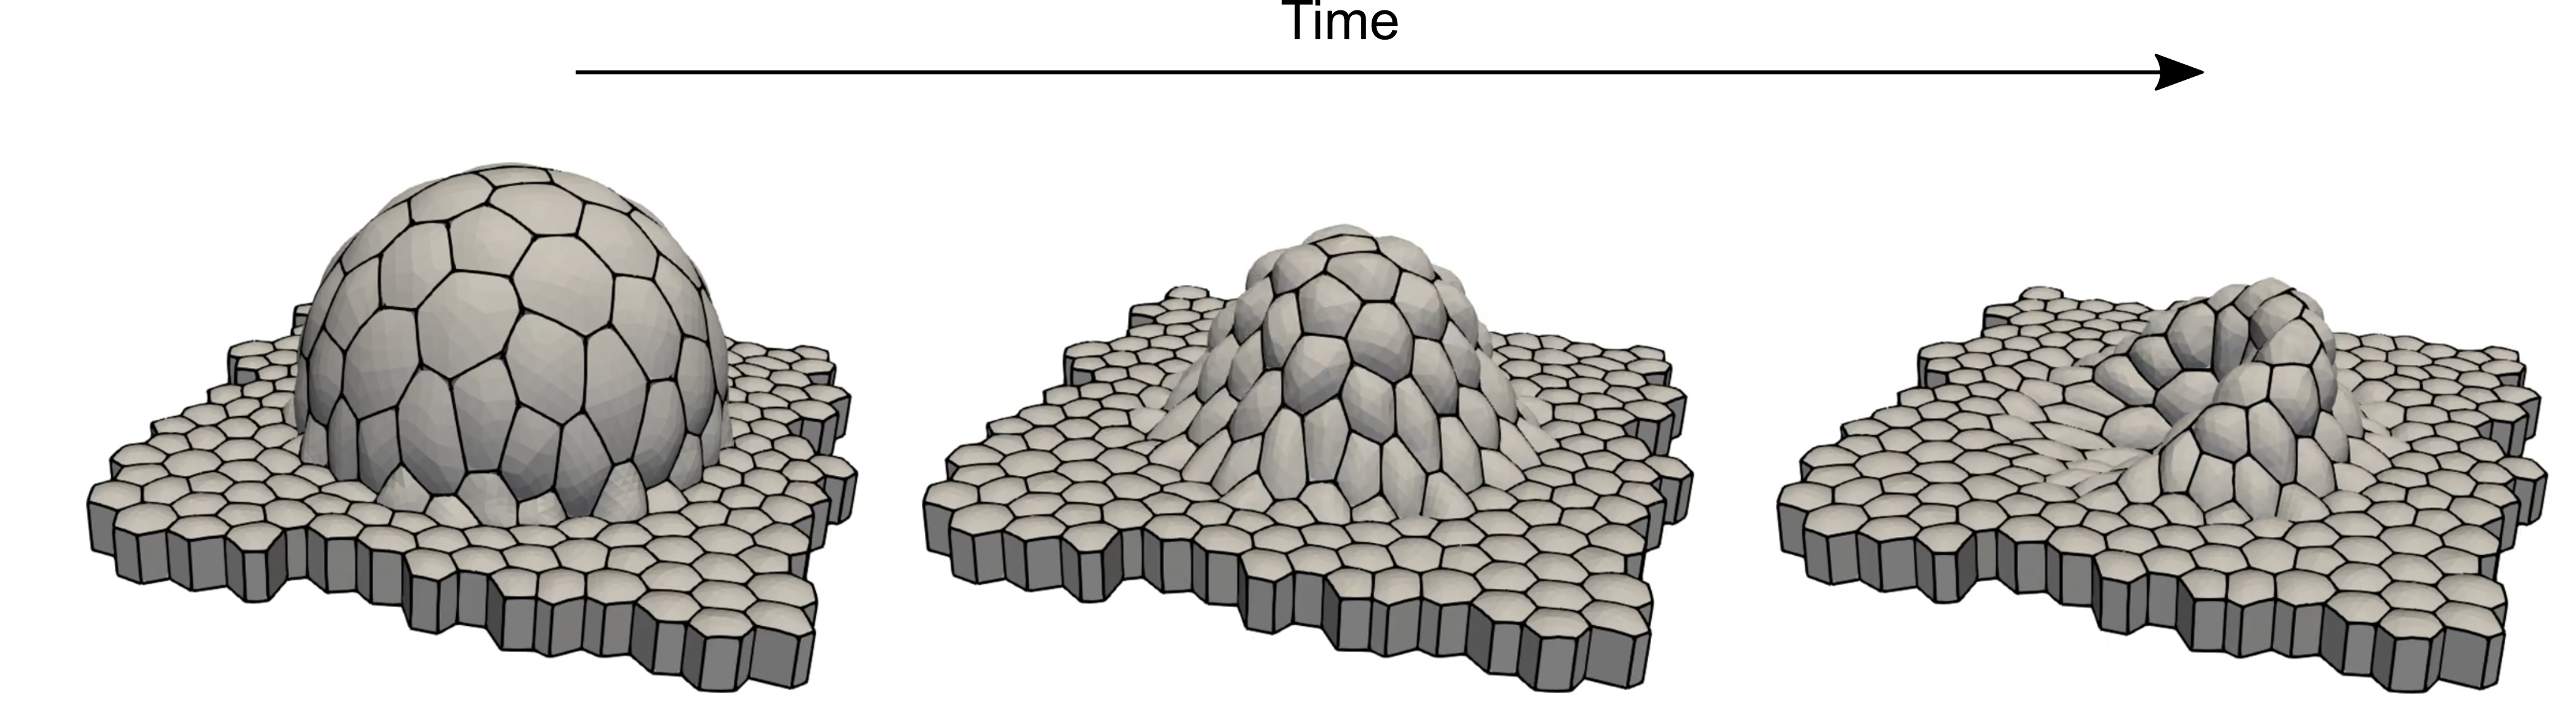
\includegraphics[width=\textwidth]{chap8_digitaldome.png}
	\caption{\label{fig_8_1} \textbf{Digital dome undergoing buckling}: A digital dome at a steady state is rapidly deflated to a negative pressure of $-50Pa$. Three snapshots show the buckling process.
	}
\end{figure}

To experimentally validate the simulation results, we designed experiments to identify the effect of hold and deflation timescales on buckling.  The pressure profiles were decided as follows (see Figure \ref{fig_8_2}):

\begin{enumerate}
	\item Initiate a linear increase in pressure from 0 to 200 Pa over a period of 10 seconds.
	\item Apply constant pressure for varying hold times, chosen based on the timescales associated with actomyosin cytoskeletal remodeling (6, 60, and 600s).
	\item Decrease the pressure to -50 Pa at varying deflation rates (0.2, 2, 20, and 200 Pa/s) which correspond to deflation times (1250, 125, 12.5, and 1.25s).
\end{enumerate}

\begin{figure}
	\begin{minipage}[c]{0.6\textwidth}
		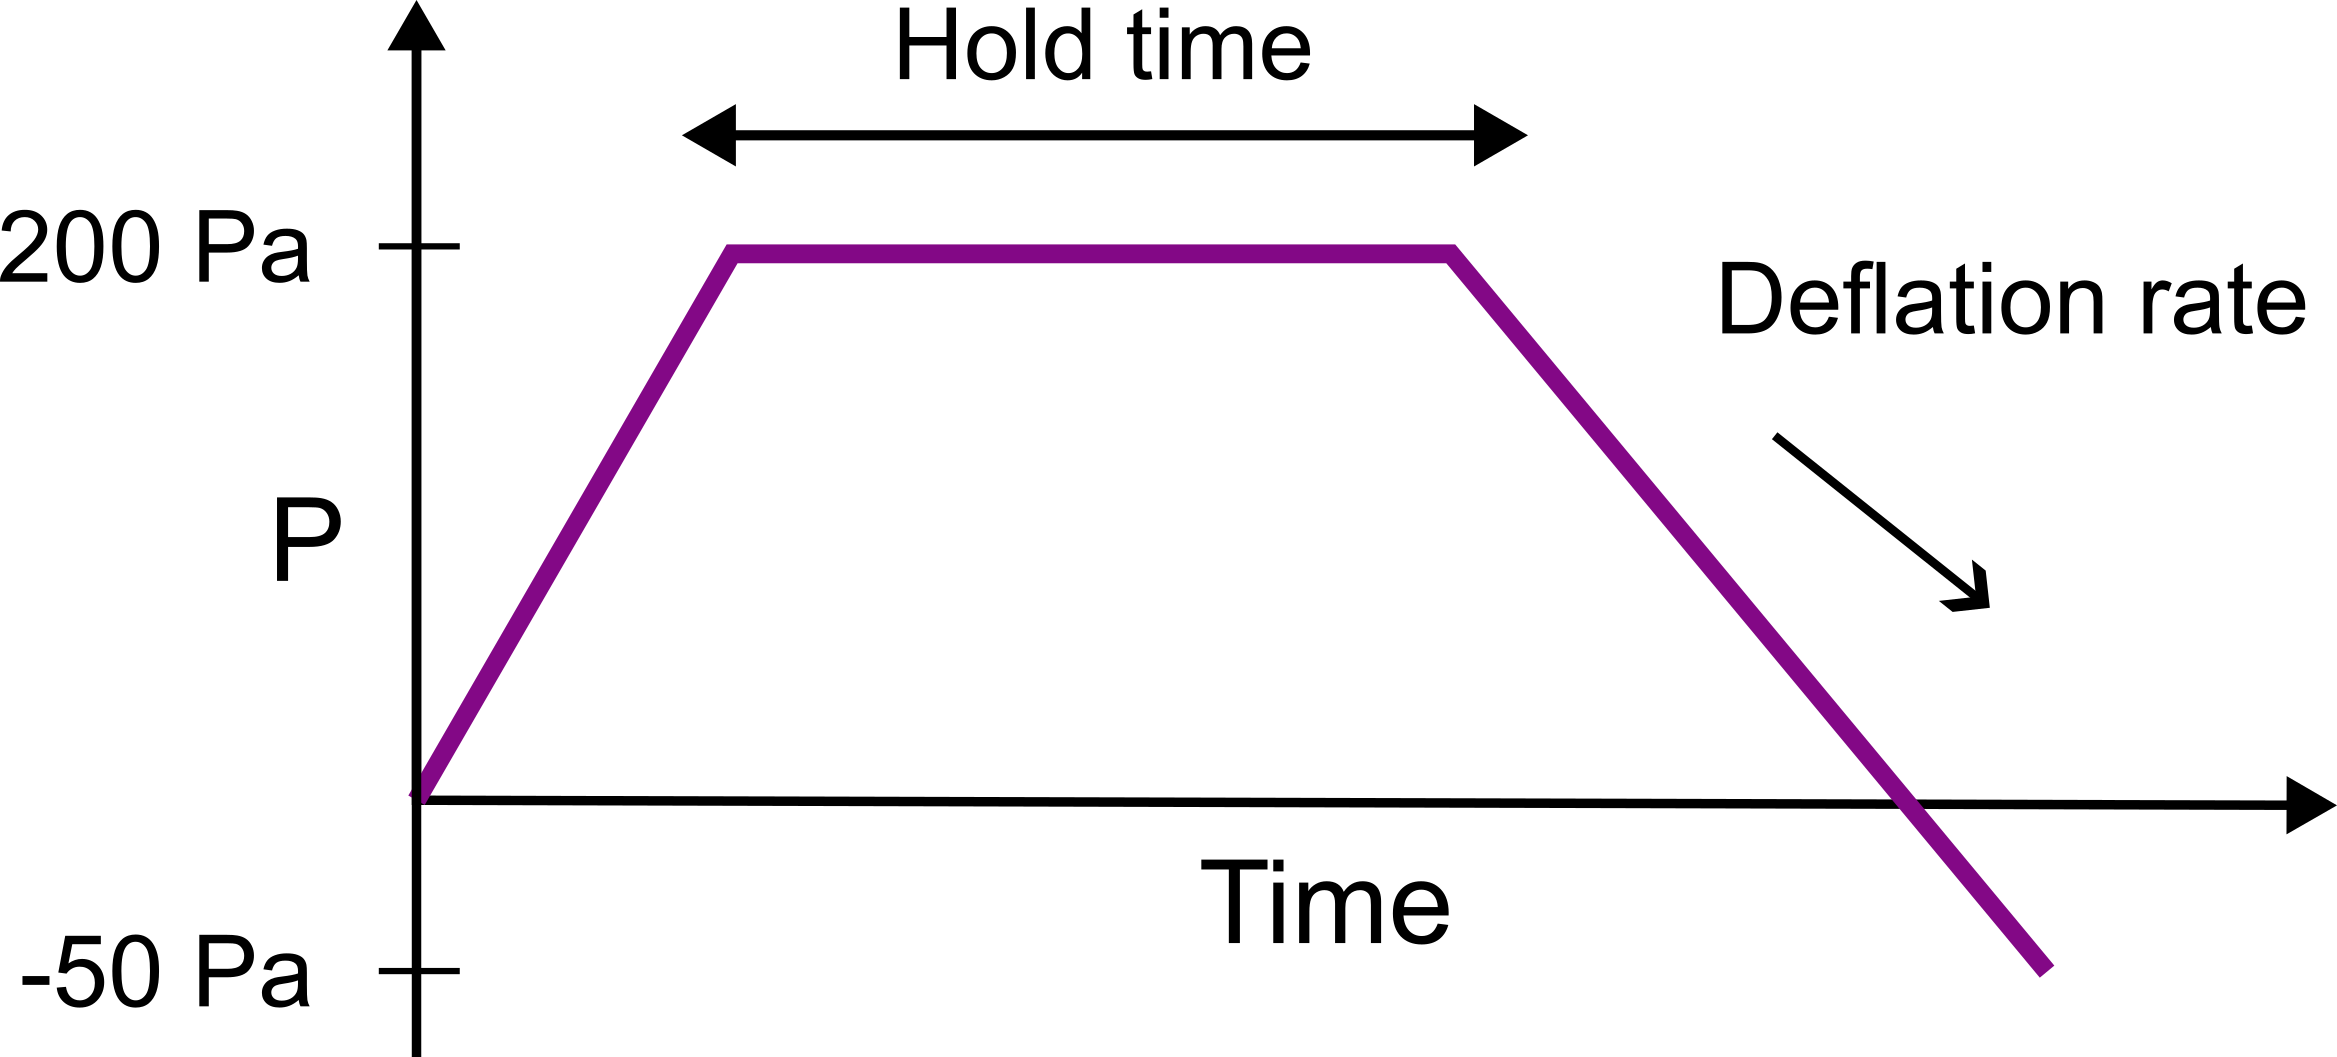
\includegraphics[width=\textwidth]{chap8_bucklingprotocol.png}
	\end{minipage}\hfill
	\begin{minipage}[c]{0.35\textwidth}
		\caption{\\ \textbf{Buckling protocol}:\\ The pressure is increased to 200Pa for inflating the dome, and then the dome is given different amounts of time (hold time) to remodel before being deflated to -50Pa at different rates (deflation rate) to observe whether the dome buckles or not.	} \label{fig_8_2}
	\end{minipage}
\end{figure}

We conducted experiments for all conditions and quantified the fraction of domes that underwent buckling. We relied on qualitative characterization of buckling events, assuming that a smooth and continuous curvature of the monolayer indicated the absence of buckling. Our results demonstrated that at the fastest deflation of 1.25s, buckling occurred for all hold times, ranging from 6s to 600s, confirming the hypothesis that rapid deflation causes buckling (see Fig. \ref{fig_8_2} A-B). In contrast, slow deflation in 1250s rarely led to buckling, irrespective of the hold time (see Fig. \ref{fig_8_2} C-D). This suggests, as the model predicted, that the tissue can effectively remodel its cytoskeleton and adapt to drastic changes in area, avoiding buckling during slow deflation.

Our findings indicate that domes subjected to a 6s hold time attained smaller strains at the end of the hold time compared to those with a 600s hold time, consistent with the results from domes subjected to constant pressure (see Fig. \ref{fig_8_2} F). We found that domes tested with longer hold times had a higher fraction of buckling domes, even for moderately slow deflation (125s). A  diagram depicting the results demonstrates the relationship between hold time, deflation rate, and the likelihood of buckling. The trend shows that as hold time increases, buckling becomes more likely at faster deflation rates (refer to Fig. \ref{fig_8_2} E). Therefore, the dome's susceptibility to buckling is influenced by the interplay between hold time, which permits cytoskeletal remodeling at constant pressure and the progressive increase of the resting area, and deflation rate, which represents the timescale at which the tissue is compressed.

\begin{figure}[b!]
	\centering
	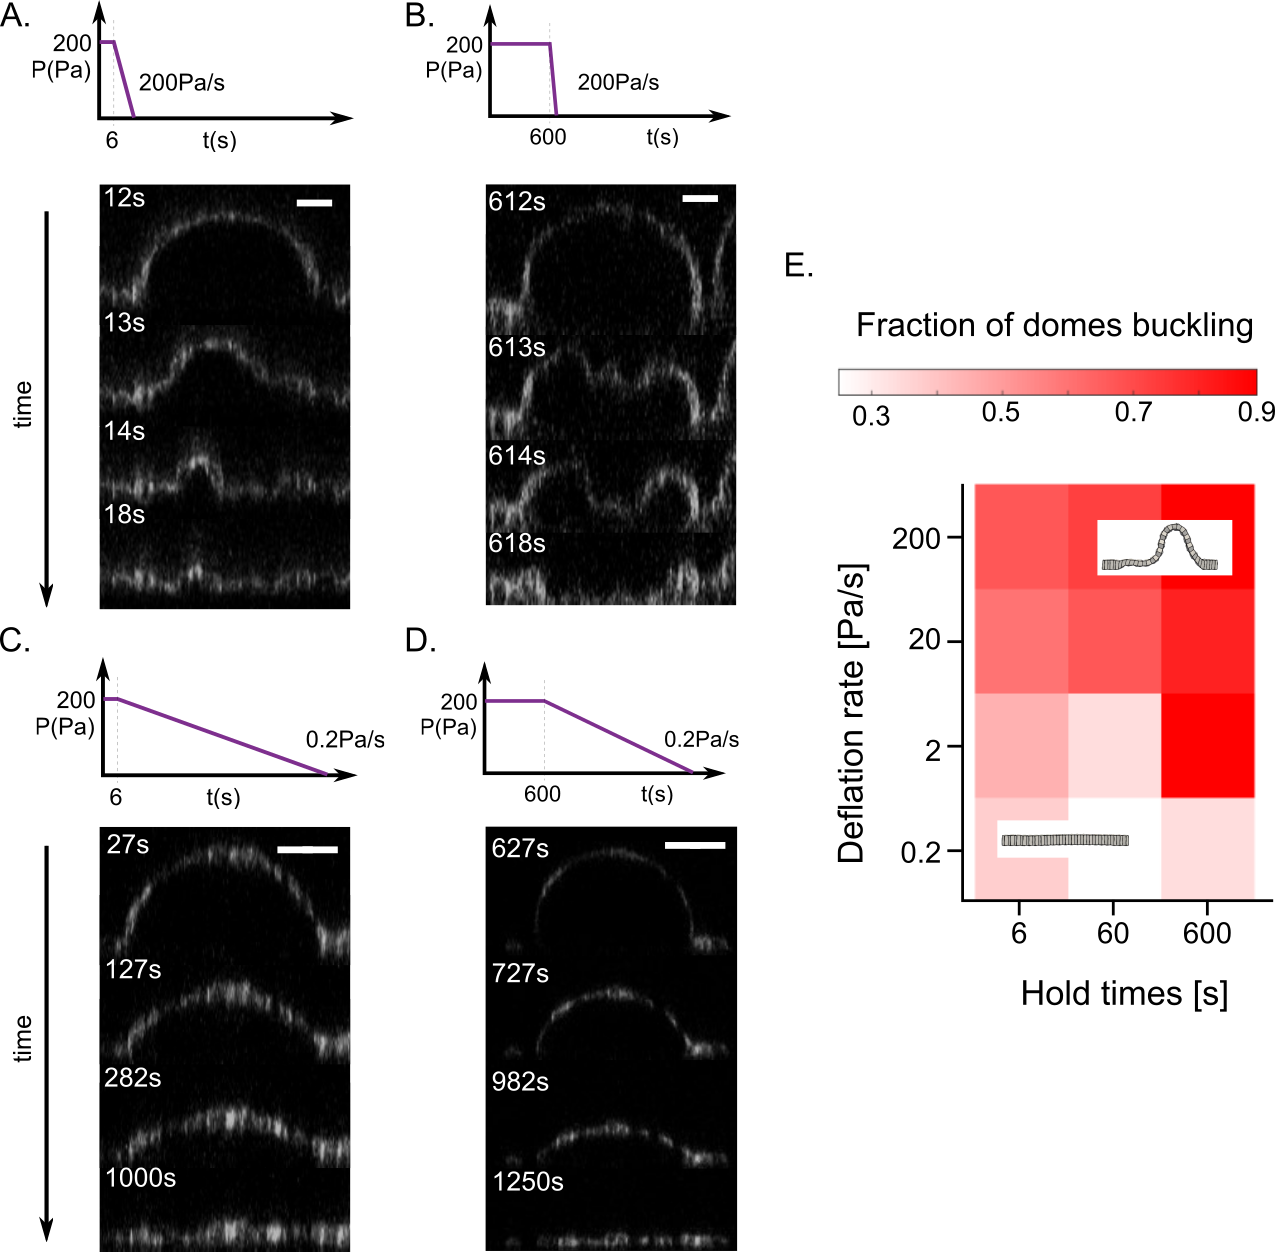
\includegraphics[width=0.95\textwidth]{chap8_buckling.png}
	\caption{\label{fig_8_3} \textbf{Buckling conditions}: (A-D) Representative montages of dome deflation for experiments and model at different deflation rates of 200 and 0.2 Pa/s after holding pressure constant of 200 Pa for 6 and 600 s. Scale bars are 20 µm for XZ. (E) Diagram representing fraction of domes buckling for different deflation rates and hold time. Showing the optimum conditions for the buckling. (F) The maximum strain achieved is lower for 6s hold time compared to 600s conditions.}
\end{figure}

Furthermore, we observed a wide variety of transient folds in the inflated buckling dome, which depended on the hold time. Buckling domes subjected to short hold times and fast deflation exhibited minor kinks in the folds, while others subjected to long hold times and fast deflation showed drastic changes in curvature (see Fig. \ref{fig_8_3} A-B).

To sum up, we experimentally validated the predictions made by the computational model that buckling in domes is a consequence of deflation being faster than cortical dynamics. In the next section, we image the buckling tissue at a higher resolution for closer look at transient folds.


\hypertarget{multiscale-buckling}{%
	\section{Multiscale buckling}\label{multiscale-buckling}}

The observation of tissue buckling was evident in the confocal line scan images. However, individual junctions are also active viscoelastic thin sheets themselves, and it has been shown that rapid contractions during morphogenesis can lead to junctional buckling \cite{Sumi:2018aa}. To examine the dynamical shape transformation during rapid deflation at multiple scales, we adapted a variation of MOLI for use with light sheet microscopy. The higher resolution 3D images of the dome revealed a variety of cell thicknesses, with thicker regions caused by the bulging of the nucleus and thin regions at the cell periphery (see Fig. \ref{fig_8_4} C).

To further investigate the phenomenon of buckling, we repeated the experiments described in the previous section, with a deflation rate of 200 Pa/s and a hold time of 600 s. Observations under the light sheet microscope revealed  additional features beyond tissue-scale buckling, including folds at cellular and subcellular scales. Upon closer inspection, we classified three levels of buckling: tissue, cellular, and subcellular.

At the tissue scale, buckling was apparent, with cells collectively transitioning from a uniform curvature to a distorted shape (see Fig. \ref{fig_8_4} A). At this level, we also observed folds occurring at the junctions between cells (see Fig. \ref{fig_8_4} B). At shorter length scales, we observed individual cells undergoing buckling (see Fig. \ref{fig_8_4} C).

In many instances, we observed buckling at even shorter length scales, which we refer to as subcellular buckling, as the folds in the membrane were distinct from the cell-level buckling. Localized folds and ruffles occurred in the thinnest parts of the stretched cells, where the membrane folded at shorter wavelengths (see Fig. \ref{fig_8_4} E). Interestingly, these folds occurred on both the apical and basal sides of the cells.

Epithelial cells have their membrane attached to the cortex through membrane-cortex attachment proteins such as ezrin, radixin, and moesin. This led us to assume that the subcellular buckling observed in our experiments is due to actin cortex buckling. To confirm this, we imaged the actin cortex while the dome was undergoing buckling using SPY actin staining, which showed that the actin cortex followed the exact shape of the membrane during buckling (see Fig. \ref{fig_8_4} G).

\begin{figure}[h!]
	\centering
	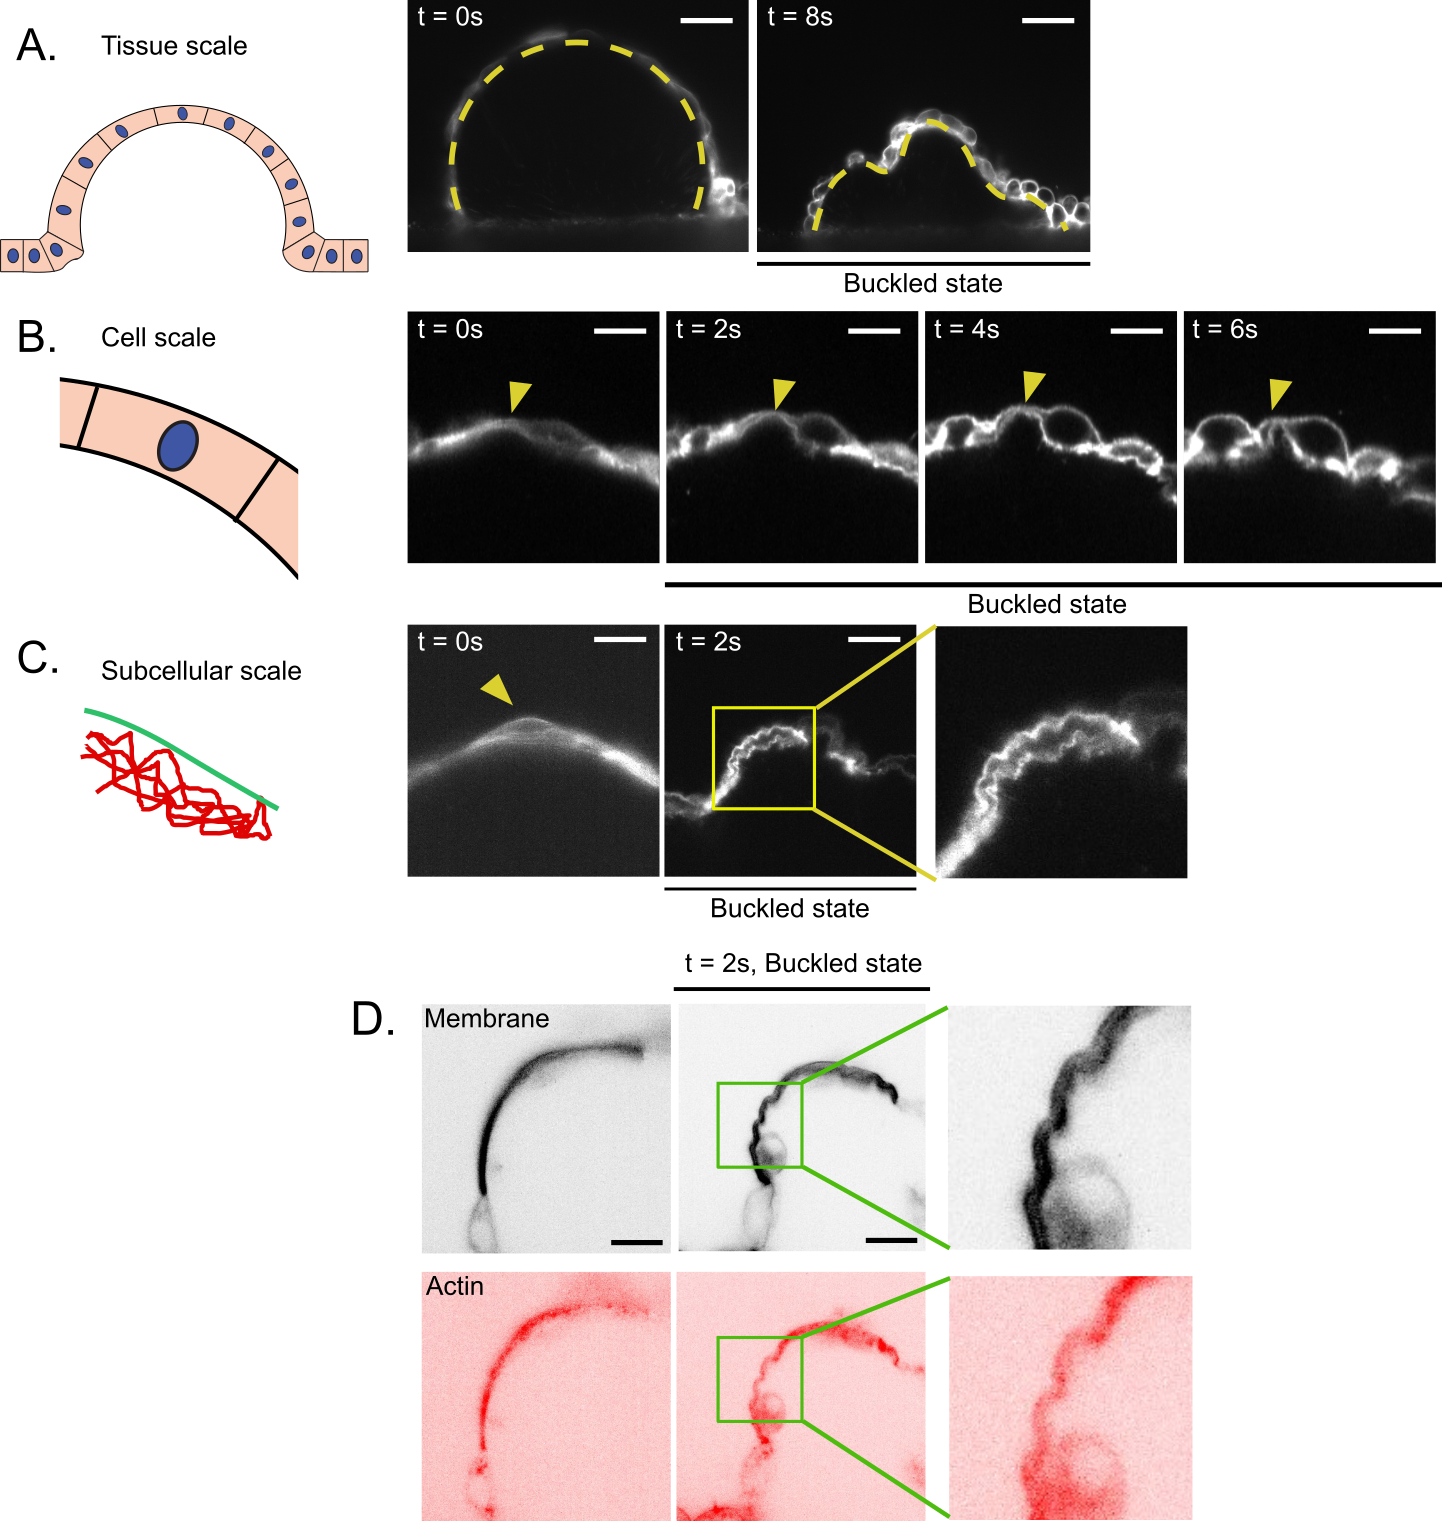
\includegraphics[width=\textwidth]{chap8_bucklingmultiscale.png}
	\caption{\label{fig_8_4} \textbf{Multiscale buckling}: (A) Midsection of a tissue dome undergoing buckling, with dotted yellow lines representing tissue curvature. Scalebar is $20\mu m$. (B) Buckling event at the cell junction where cells buckle at a shorter length scale. (C) Localized subcellular buckling in a single cell with varying thickness from the nucleus to the periphery. (D) Buckling at the cellular level but not at the tissue level. Scalebar is $20\mu m$. (E) Subcellular buckling resulting in the formation of ruffles at short wavelengths (inset). Scalebar is $5 \mu m$. (F) Buckling occurring at the subcellular level. Scalebar is $20\mu m$ with an inset scalebar of $5 \mu m$. (G) Cross-sections of the membrane and actin in cells undergoing subcellular buckling. Scalebar is $5\mu m$. (H) Region of tissue undergoing buckling at multiple length scales. Scalebar is $5\mu m$ for (C,E,G,H).}
\end{figure}

Moreover, we found that while some domes were not buckling at the tissue scale, they were still exhibiting buckling at the cell or subcellular level (see Fig.  \ref{fig_8_4} D F). Furthermore, we found instances of simultaneous buckling at multiple length scales (refer to Fig. \ref{fig_8_4} H), indicating that these categories are not mutually exclusive.

In summary, our observations of tissue buckling, cellular buckling, and subcellular buckling provide new insights into the mechanics of epithelial tissues. The hierarchical architecture of these biological interfaces is mirrored by a hierarchy of buckling scales. Each of these buckling scales provide distinct mechanisms to release compressive stresses in cortical surfaces. 

\hypertarget{generating-epithelial-folds}{%
	\section{Generating epithelial
		folds}\label{generating-epithelial-folds}}

In this section, we explored the formation of epithelial folds after deflation. During deflation, we observed the tissue making contact with the substrate in certain regions first, leading to the formation of folds in the regions where it made contact last (see Fig. \ref{fig_8_6} A-C). To investigate if there was any pattern to these folds, we examined buckling of spherical domes of different sizes. Indeed, larger domes result in more slender structures, known to exhibit more intricate buckling patterns. Our observations revealed two types of folding patterns emerging: accumulation along the periphery and folds in the middle (see Fig. \ref{fig_8_5}).

\begin{figure}[h!]
	\begin{minipage}[c]{0.5\textwidth}
		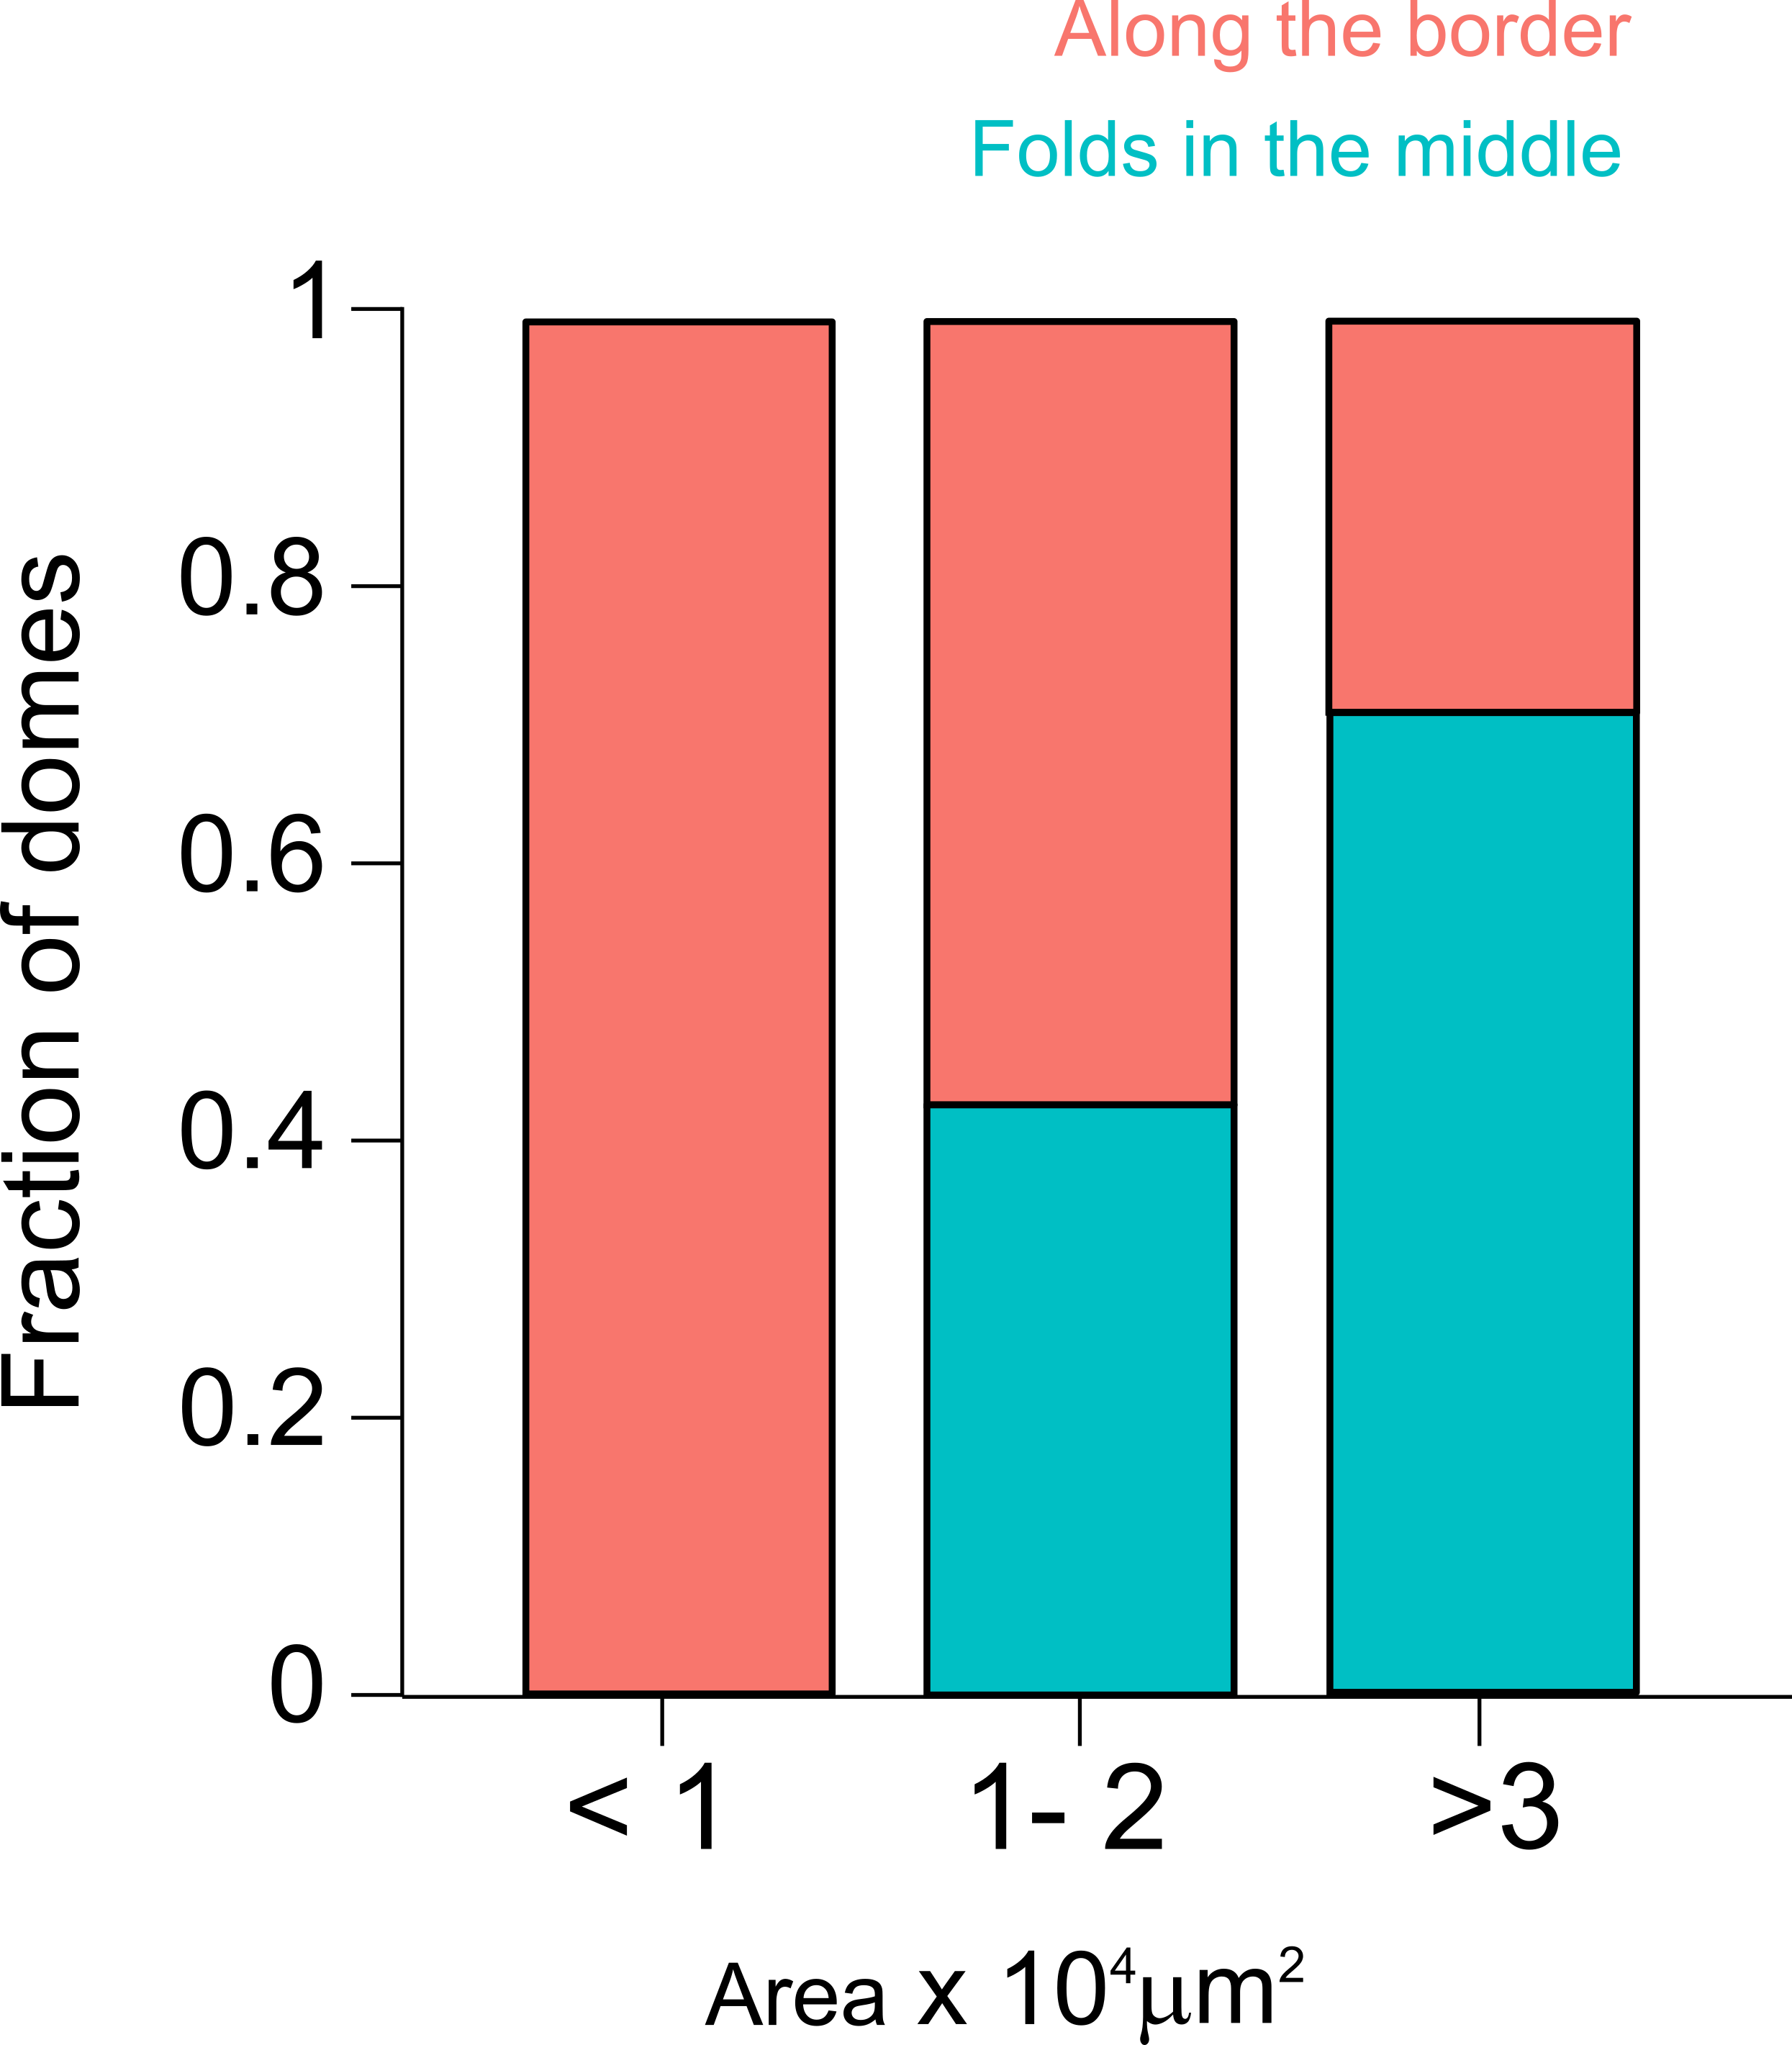
\includegraphics[width=0.8\textwidth]{chap8patternfraction.png}
	\end{minipage}\hfill
	\begin{minipage}[c]{0.45\textwidth}
		\caption{\\ \textbf{Buckling patterns}:\\ 
			Buckling patterns observed in differently sized digital domes. The domes were grouped into three size categories and two categories based on location of folds (along the border and in the middle). We found that larger domes are more likely to buckle into a network of folds compared to smaller ones.
		} \label{fig_8_5}
	\end{minipage}
\end{figure}

For smaller domes with a footprint diameter smaller than 110 \unit{\um}, we repeatedly observed that most of the buckling resulted in an accumulation around the periphery (see Fig. \ref{fig_8_6} A). The confocal time-lapse from the base gave the impression of an annular structure, but three-dimensional imaging of the folds revealed a crescent-shaped fold, taller on one side than the other. For larger domes with a footprint diameter greater than 300 \unit{\um}, we observed instances of domes forming a network of folds in the middle, with multiple folds connecting each other by forming junctions (see Fig. \ref{fig_8_6} C). Finally, for intermediate-sized domes, we observed a mixture of accumulation and folds, although the proportion of folds along the periphery decreased (see Fig. \ref{fig_8_5} ).

\begin{figure}[h!]
	\centering
	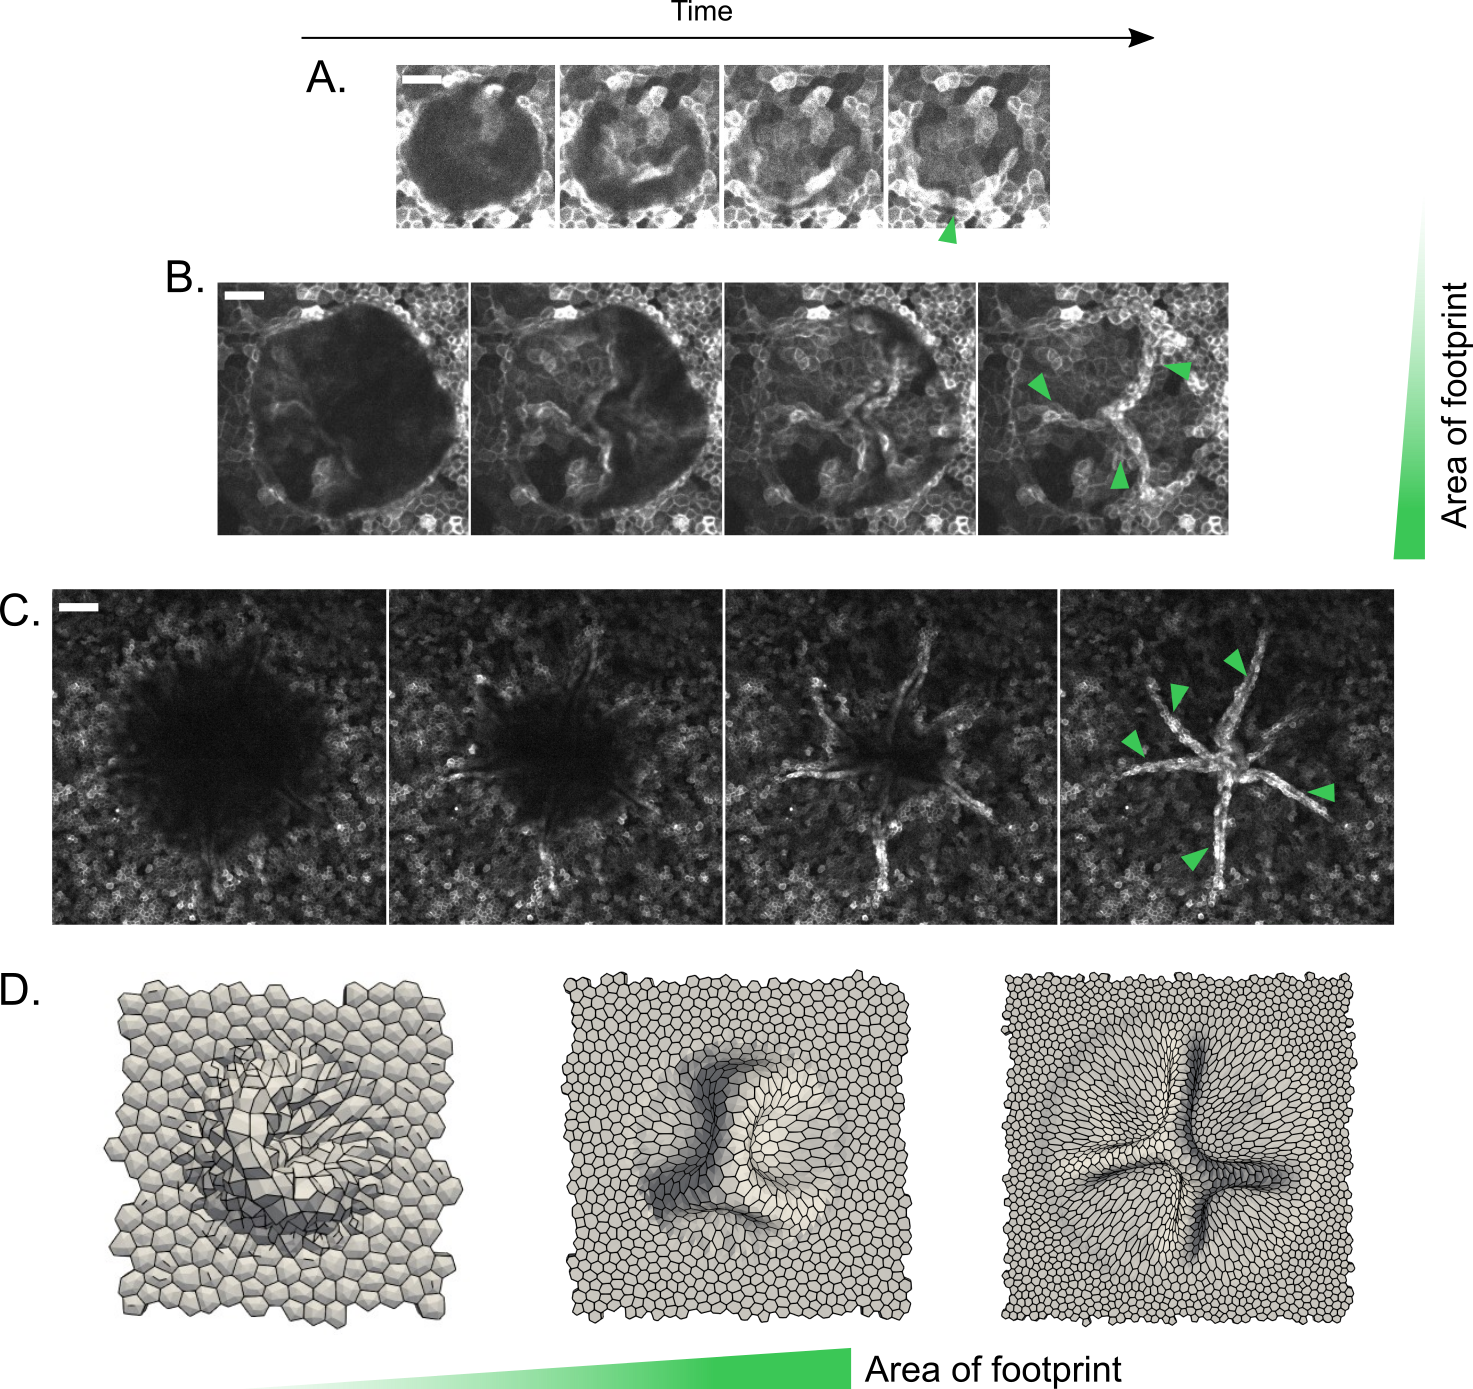
\includegraphics[width=\textwidth]{chap8_bucklingfolds.png}
	\caption{\label{fig_8_6} \textbf{Buckling patterns in spherical domes of varied size}: Representative examples of digital domes undergoing buckling with time-lapse of their basal cross-section (A-C). In the first frame, the onset of buckling is visible where the dome makes contact in the middle. Subsequent frames show more of the fold coming into view, and when the dome completely deflates, a fold is formed (indicated by the green arrow). Panel (D) shows the final outcome of buckling for digital domes of different sizes. Scale bar is $20 \mu m$	}
\end{figure}
\clearpage

We also observed the same folding patterns in the digital domes when performing the same deflation experiments (see Fig. \ref{fig_8_6} D). Larger digital domes produced more radial folds, and smaller ones formed an accumulation on the side. Intermediate-sized digital domes showed a mixture of both patterns.
Our findings suggest that the folding patterns may be governed by the size and shape of the dome. In the next section, we will attempt to control the folds by controlling the footprint shape.

\hypertarget{forming-predictable-folds}{%
	\section{Forming predictable folds}\label{forming-predictable-folds}}

In this section, we explore the formation of predictable folds by deflating epithelial domes. While size provides some degree of control on the buckling pattern of spherical domes, because of their high symmetry and the characteristic symmetry-breaking of buckling patterns, the geometry of the resulting folds is very difficult to control. To break symmetry and guide buckling, we generated large digital domes of the same footprint area but with distinct geometries, including an ellipsoidal and a triangular shape. Remarkably, we found that the digital domes buckled into predictable patterns, with the ellipsoidal shape forming a line along the major axis and the triangular shape forming a Y-shaped network of folds.

To test the dependence of shape and size on folds, we conducted experiments using MOLI with ellipsoidal domes of varying sizes. Our observations revealed that larger ellipsoidal domes buckle into a fold along their major axis, just like digital domes, while smaller ellipsoidal domes produced a similar peripheral accumulation as spherical domes (see Fig \ref{fig_8_7} A). This suggests that only larger domes, regardless of their shape, possess the capability to produce folds in the middle.
 
Furthermore, we found that triangular domes buckled into a Y-shaped network of folds that resembled the pattern observed in digital domes (see Fig \ref{fig_8_7} D). The timelapse of buckling indicated that the vertices of the triangular domes pushed the buckling along the medians of the triangle (see Fig \ref{fig_8_7} C).

We observed that the folds exhibited variability in terms of stability, with some dissipating into a the monolayer while others remaining intact and even forming attachments with each other.  These folded structures were stable for several hours and could be imaged for over 12 hours (see Fig \ref{fig_8_7} E-F). Interestingly, when immediately inflated, these folds would unfurl into a smooth dome again.

Our results suggest that the MOLI system could provide a novel way of generating epithelial folds, with potential applications in tissue engineering. These results demonstrate that by controlling a few mechanical parameters such as geometry and pressure, it is possible to harness active viscoelasticity and  buckling to program epithelial folds.

\begin{figure}[h!]
	\centering
	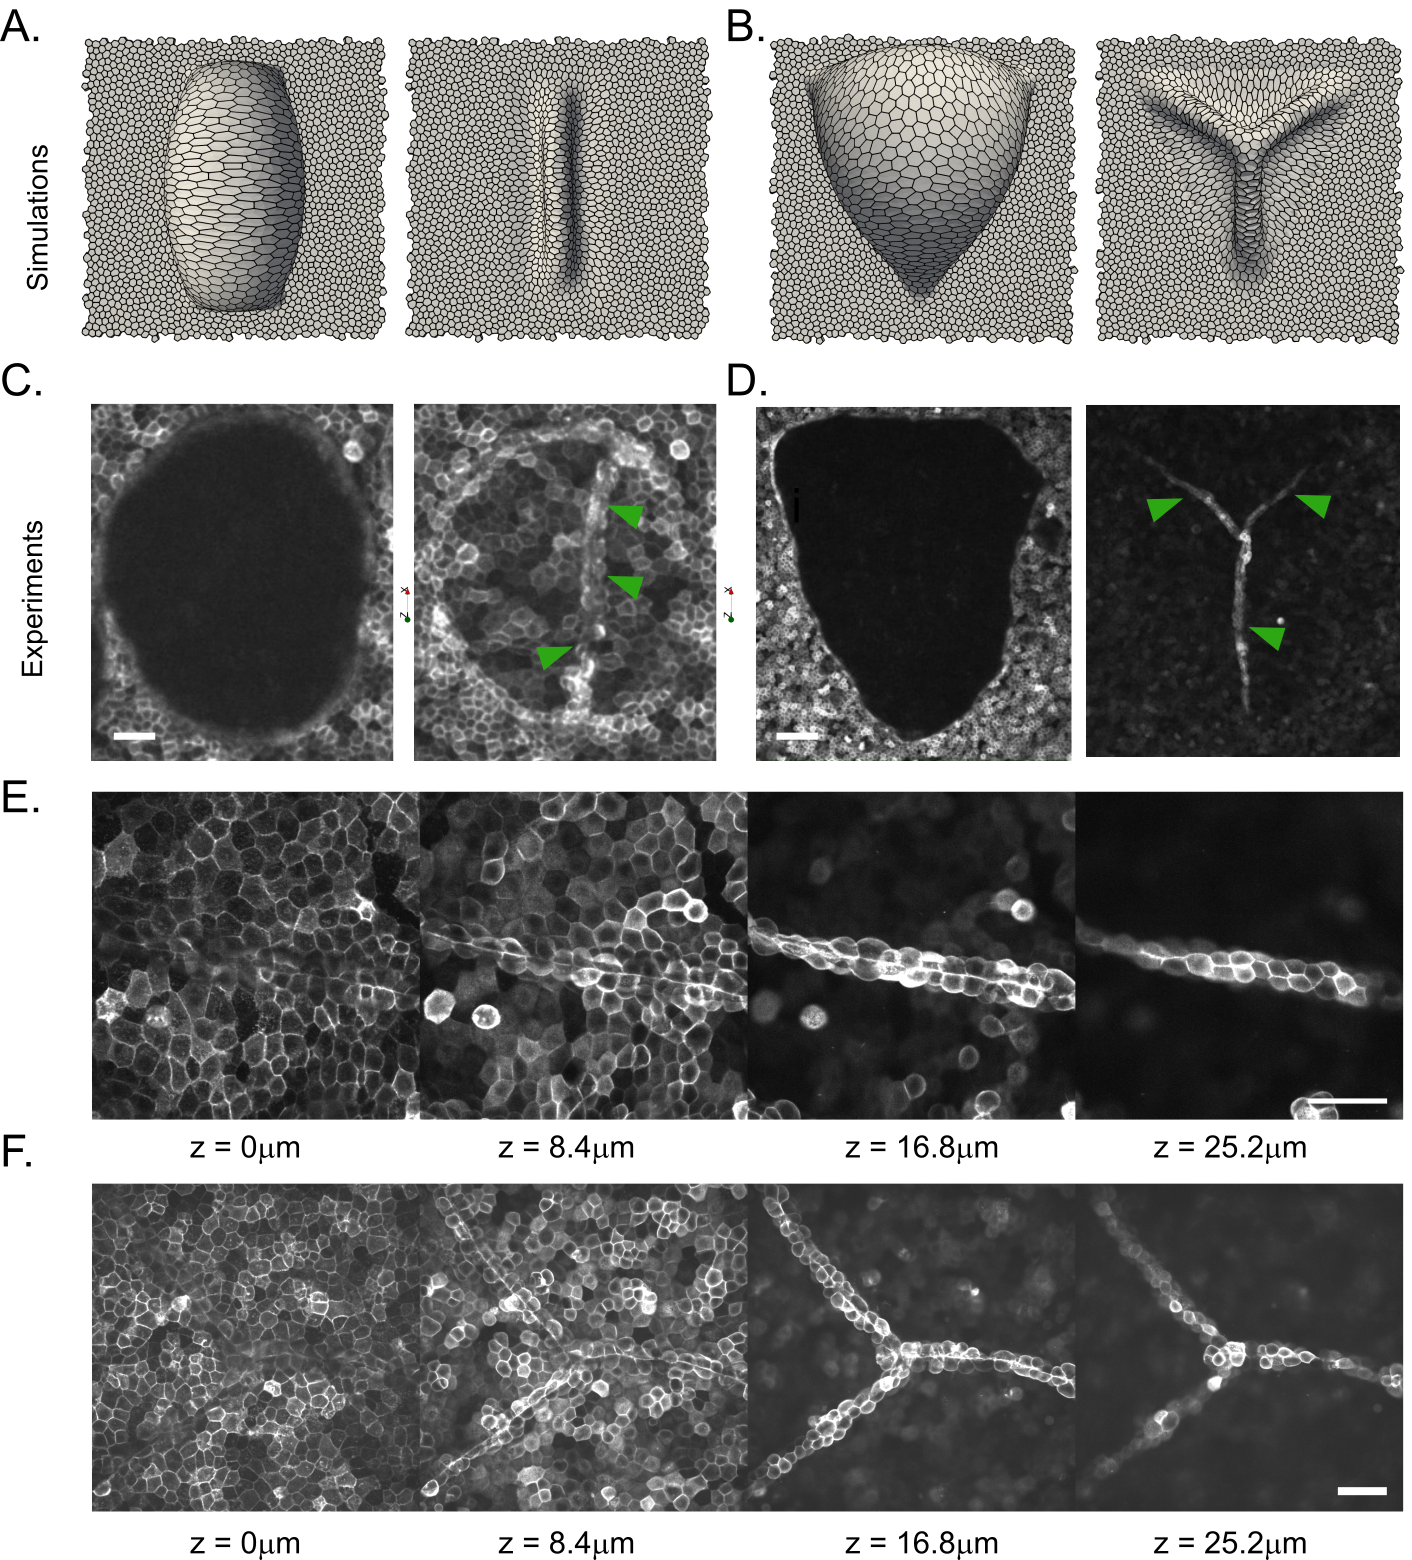
\includegraphics[width=\textwidth]{chap8_pfolds.png}
	\caption{\label{fig_8_7} \textbf{Controling the patterns of fold}: A-B Simulations show digital models of ellipsoidal and triangular domes buckled into line and Y-shaped junctions. C-D Experimental results confirm the simulation findings. E-F Confocal z-stack images show the folds in the case of a line and Y-shaped junction. Scale bar is $50\mu m$.	}
\end{figure}


%\newpage

\hypertarget{summary-and-discussion-1}{%
	\section{Summary and Discussion}\label{summary-and-discussion-1}}

In this chapter, we investigated the buckling response of epithelial tissue to deflation and its relationship with actin remodeling timescales. We utilized our device to generate domes from flat monolayers and observed buckling occurring at various scales, from the tissue level down to the actin cortex of individual cells. Our results revealed that buckling is triggered when deflation occurs more rapidly than actin can remodel. We also explored the patterns of folding that emerge from differently sized and shaped domes and proposed a novel method of creating controlled folds from planar monolayers. With the aid of computational models, we demonstrated the engineering potential of the dome system to produce structured folds by manipulating footprint geometry and pressure.

The prevalence of mechanical instabilities in biological systems is well established, and buckling in MDCK epithelial monolayers has been observed through various methods, including growth in confinement or direct compression \cite{wyatt2020,trushko2020}. Wyatt et al. demonstrated that uniaxial compression beyond 35\% strain can cause epithelial monolayers to buckle out of plane, and active contractility can recover the deformation within tens of seconds depending on the degree of compression. These buckles were essentially one-dimensional, whereas our study allows us to examine the much more challenging situation of biaxial buckling. We further provides mechanistic insights into the buckling process and its implications for tissue architecture at multiple scales, which has not been previously explored. 

Our results highlight the hierarchical structure of epithelial tissue, which is composed of various components that sustain deformations and forces at different levels. The actin cytoskeleton plays a crucial role in defining the shape of cells and tissues at multiple scales \cite{clarke2021}. A cell monolayer can be viewed as an assembly of cells with their own surface tension and material properties, implying that a material with different length scales would buckle at different length scales. The conditions under which a tissue releases compressive stresses at a given scale and the biological consequences remain to be understood. 

The short-wavelength folds resulting from subcellular buckling are an intriguing aspect to consider. It is important to note that actin buckling is not a novel phenomenon, and minimal models of actin filaments with myosin motors on a lipid membrane have demonstrated that myosin-induced contraction leads to actin filament buckling \cite{murrell2012, costa2002,  wang2019}. Researchers have also reported multiple modes of buckling and wrinkling in membrane-actin droplets, depending on the thickness \cite{kusters2019}. Interestingly, they found that thin shells undergo buckling and produce wrinkles in the membrane but not in actin, indicating the possibility of different modes of buckling within a cell, which is closely related to what we observed in our experiments. In the future, faster 3D confocal imaging could enable further quantitative analysis of these transient folds.

Our findings on tissue-scale buckling can be related to modes of buckling in thin shells. Our computational model suggests that the cortex behaves like a hyperelastic material at short timescales, as in our case, where the tissues are deflated at a rapid rate. Analogous results can be expected if we repeated the experiment with elastic shells. Elastic shell buckling exhibits similar aspects, including the folds and patterns that emerge when different sized shells buckle. Localized defects engineered in the shells can also influence the sensitivity of buckling pressure \cite{lee2016a}. We speculate that the non-uniform thickness of the cells, with thicker regions near the nucleus and thinner regions at the edges, provide the defects in thin shell geometry that result in localized folds. Future studies that quantify the relationship between the shell thickness and the emergence of folds may shed light on the precise mechanisms underlying the formation of subcellular folds in our experiments.

The slenderness, defined as the ratio of dome radius to thickness, provides a guide to understanding the different modes of buckling. Shells with high slenderness ratios are expected to exhibit higher modes of buckling compared to thicker shells. However, our experiments go beyond mere understanding of the system and demonstrate that we can program folds by controlling two parameters: geometry and pressure. For non-spherical domes, anisotropic stresses are observed along the axes of the elliptical footprint for ellipsoidal domes \cite{marin-llaurado2022}. These stresses can orient the folding in a particular direction to generate a programmed fold, such as Y junctions on the sides of a rectangular footprint. A recent study has shown that confining elastic shells in smaller areas produces orderly wrinkles that depend on the curvature of the shell, which can be predicted by analytical solutions \cite{tobasco2022}. We note however that the predicted orientations of folds are orthogonal to those in our domes, highlighting the subtlety of predicting wrinkle patterns. Further advances in understanding the geometric and mechanical rules that control wrinkling patterns, combined with our experimental results, may offer insights into future tissue engineering applications.

In summary, this thesis presents a novel experimental system that facilitates the generation of epithelial domes and their subsequent transformation into folds by deflation. Our findings reveal that the timescales of actomyosin cytoskeleton remodeling are critical in this transformation process. Through the manipulation of epithelial geometry and deflation rate, we demonstrate that it is possible to engineer epithelial folds with desired geometry. The results of our study may have important implications for tissue engineering and the development of new techniques for controlling epithelial architecture.